\subsection{Evaluating Performance Comparison Results}

\textbf{COHEN: How did the program performance compare to its selected standard?} 
\textbf{Did the program demonstrate good performance?}
\textbf{Is the programs performance different from predictions?} 
\textbf{Did you learn what you wanted from the experiments?}

The best route set, having four routes, constructed by the proposed algorithm (SSO) is presented in Table \vref{table:performanceComparison_bestRouteSet4} and illustrated in Fig. \vref{fig:bestRouteSet4}. The best route set, having four routes, constructed by a plain ACO implementation is found in Table \vref{table:performanceComparison_bestRouteSet4_ACO}. The best, worst, average, median produced results with the standard deviation can be found in Appendix \ref{appendixC}, Table \vref{table:performanceComparison_ACOFull}. 

As seen in \vref{table:performanceComparison_ACOSSOBEST}, the SSO performs overall better than the plain ACO implementation. In ACO, compared to SSO, the ants do not possess memory, which enables ants to ``remember'' nodes visited within the same route set. Constraint \vref{itm:criteriaConnectedGraph} states that the produced route network must be connected, and without the memory feature ACO will produce less route sets that satisfies this constraint.  ACO also has, as mentioned, a known limitation of getting stuck at a local optima. This disadvantage is demonstrated in Figure \ref{fig:acovssso}, which shows the average growth in the $TOTFIT$ value for each iteration, of both algorithms. The algorithms are run 10 times, and for each iteration the average $TOTFIT$ value for each run is recorded. As one can observe, the ACO implementation manage to find good solutions fast, by following pheromone trails laid by previous ants. However, after approximately 35 iterations, the algorithm does not discover better solutions. The amount of pheromone on the initial first best routes continue to increase, and with this unable the next ants to explore possible better routes. As one can see, the proposed SSO algorithm manage to get out of this inconvenience. As we observed in the parameter settings results, found in Table \vref{table:pm2}, the additional $CA$ and $AF$ parameters both improved the $TOTFIT$ value. The amount of $CA$ enables the algorithm to explore new, possible better, routes, regardless of the pheromone value laid on the edges. This parameter can therefore enable the algorithm to get out of a local optima. The reader recalls that the $AF$ parameter selects the best produced route sets after an iteration, and the same amount of following ants will basically reward these edges with more pheromone. As also observed in the parameter settings results, was that giving these best roots additional pheromone improved the $TOTFIT$ value. 

In addition, will rewarding edges in an iteration' best route sets with more pheromone boost good routes. As we also observed in the PM, laying a high amount of pheromone on these edges increased the $TOTFIT$ value. If a better global best solution is found, it updates the global best solution, and increase the possibility of the next ants to select the edges walked in it's routes. 

%As one also can observe, the difference in $ATT$ is less than the difference in $d_0$. The ACO increase the pheromone trail of short routes, which reflects the average travel time in the route set. A satisfied passenger also involves a minimum number of transfers. And the SSO takes this to consideration, when seeing the big picture in the best produced route sets.

 \begin{figure}[H]
    \begin{center}
    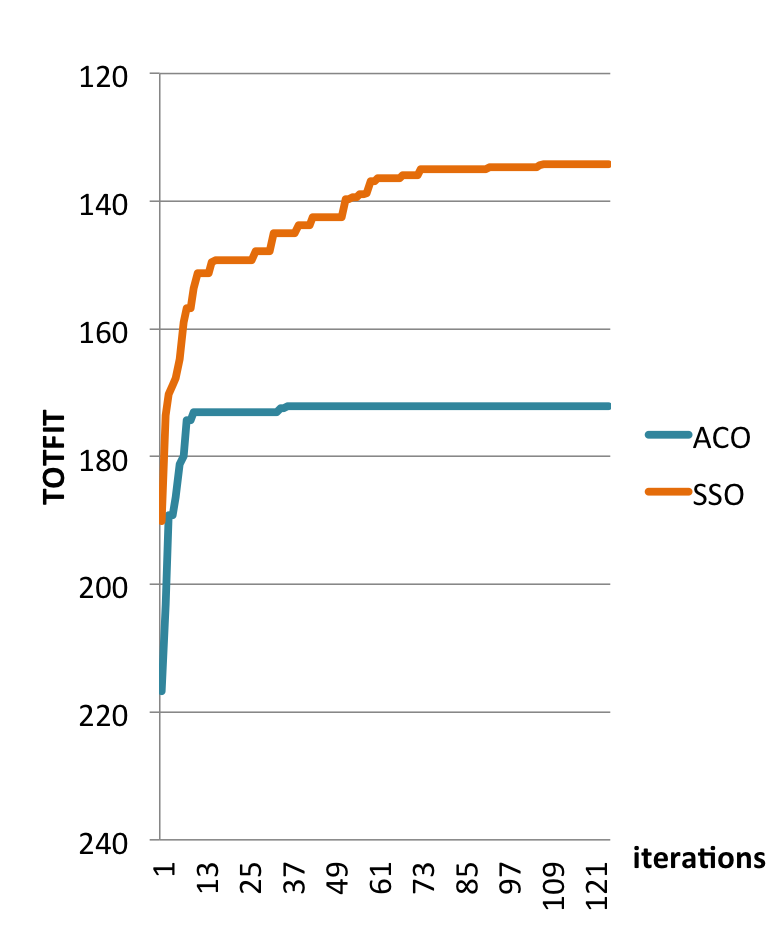
\includegraphics[width=3in]{assets/acovsssoNEW.png}
    \end{center}
    \caption{Evolution of TOTFIT for ACO and SSO }
    \label{fig:acovssso} 
\end{figure}

In Table \vref{table:performanceComparison_4}, the results of the SSO, having four routes, are compared with the respective experimental results published in the literature. As presented in Table \vref{table:performanceComparison_4}, the route set constructed by SSO has lower ATT compared to all route sets constructed by other approaches. The values of the rest of the performance criteria $d_0, d_1, d_2, d_{unstat}$, route sets constructed by almost all, except \citep{mandl79, kidwai98, chakroborty02}, produce better results concerning number direct travelers. 

The low value of ATT is due to the weighting parameter of f.. The other approaches has sat this to favor d0 - leses mer om dette. This is due to the user set parameters is .. and ATT is favored against traveling directly. In the other \emph{\color{blue} TODO} the weights for parameters F1, F2 and F3, which together is the TOTFIT value, is weighted the same. The best produced TOTFIT, does not mean it only selects route sets with the lowest ATT, it will still select the once with one of the best produced d0. But the ratio against these two parameters favourise a low ATT against a low d0. The weight parameter, $\sigma$, explained in \vref{sec:f1}, is a user defined parameter used to control the importance of $Fi$. In this solution this is sat to favor $ATT$. This is demonstrated in Fig. [som skal lages], When traveling from node7 to node14 the passenger would have to change route from route 4 to route 3 at node 10 and the traveling time will be 20 mins including transfer penalties. If the algorithm would favour route 1, which travels dirctly from node 7 to node 14, the traveling time would be 27 minutes - increasing the ATT.

The best route set, having six routes, constructed by the proposed algorithm is presented in Table \vref{table:performanceComparison_bestRouteSet6} and Fig. \vref{fig:bestRouteSet6}. 
Evaluate.

The best route set, having seven routes, constructed by the proposed algorithm is presented in Table \vref{table:performanceComparison_bestRouteSet7} and Fig. \vref{fig:bestRouteSet7}. 
Evaluate

The best route set, having eight routes, constructed by the proposed algorithm is presented in Table \vref{table:performanceComparison_bestRouteSet8} and Fig. \vref{fig:bestRouteSet8}.
Evaluate

As one can observe in \vref{table:performanceComparison_routesets}, the amount of direct travelers increase with in line with the number of route sets. This makes sense because thus more route sets the passenger can choose from, thus bigger probability for the passenger to find a route that is convenient for him / her. This is well demonstrated when comparing the graphs of four route sets, \vref{fig:bestRouteSet4}, and six route sets, Figure \vref{fig:bestRouteSet6}, and seven route sets. However, as one can see in route sets eight. It has reached a threshold \emph{\color{blue} TODO: må vente på resultater fra sso8}.

 \begin{table}[H]
    \centering
    \begin{tabular}{|l||l|l|l|l|l|}
    \hline
    Route Set & $d_0(\%)$ & $d_1(\%)$ & $d_2(\%)$ & $d_{unsat}(\%)$ & $ATT$ \\
    \hline
    4 & 85.21 & 13.49 & 1.30 & 0.00 & 10.27\\
    6 & 87.17 & 12.0 & 0.82 & 0.01 & 10.11\\
    7 & 88.49 & 10.72 & 0.79 & 0.0 & 10.08\\
    8\\
    \hline
    \end{tabular}
    \caption {Evaluating increase of Route Sets}
    % 50 runs
    \label{table:performanceComparison_routesets}
\end{table}

